%% Calibrating Perturbation Controls for EEG Decoder Audits
%% ICAISE 2026 single-column manuscript (ACM Primary Article Template).
\documentclass[manuscript,nonacm]{acmart}
\usepackage{paperstyle}

\graphicspath{{figures/}}

%% The template numbers its references, so override acmart's author-year default.
\citestyle{acmnumeric}

\begin{document}

\title{The Control Is the Instrument}
\subtitle{Calibrating Perturbation Tests Used as Evidence That EEG Decoders Read
Neural Signal}

\author{Isha Gupta}
\equalcontrib
\affiliation{%
  \institution{Nexus Labs}
  \city{Palo Alto}
  \state{California}
  \country{USA}}

\author{Ishaan Mohandas}
\equalcontribmark
\affiliation{%
  \institution{Nexus Labs}
  \city{Palo Alto}
  \state{California}
  \country{USA}}

\author{Ashwath Raghu}
\equalcontribmark
\affiliation{%
  \institution{Nexus Labs}
  \city{Palo Alto}
  \state{California}
  \country{USA}}

\author{Jake Rajbhandari}
\equalcontribmark
\affiliation{%
  \institution{Nexus Labs}
  \city{Palo Alto}
  \state{California}
  \country{USA}}

\author{Anya Samuel}
\equalcontribmark
\affiliation{%
  \institution{Nexus Labs}
  \city{Palo Alto}
  \state{California}
  \country{USA}}

\author{Riva Sheth}
\equalcontribmark
\affiliation{%
  \institution{Nexus Labs}
  \city{Palo Alto}
  \state{California}
  \country{USA}}

\author{Mridhula Suresh}
\equalcontribmark
\affiliation{%
  \institution{Nexus Labs}
  \city{Palo Alto}
  \state{California}
  \country{USA}}

\author{Srikanth Samy}
\affiliation{%
  \institution{University of California, Berkeley}
  \city{Berkeley}
  \state{California}
  \country{USA}}
\email{ssamy@berkeley.edu}

\author{Ishaan Gupta}
\affiliation{%
  \institution{Stanford University}
  \city{Stanford}
  \state{California}
  \country{USA}}
\email{ishaangupta@stanford.edu}

\begin{abstract}
A standard argument in brain--computer-interface research runs: we removed the $\mu$
band, accuracy dropped, therefore the decoder uses sensorimotor rhythm. The argument is
valid only if the perturbation has known sensitivity and, critically, a known
false-alarm rate for the decoder being tested. Almost no published perturbation control
has been characterised that way. We treat controls as measuring instruments and
calibrate them against operational ground truth. Using a simulator in which the signal
is planted by construction, we measure each control's catch rate and false-alarm rate
across a grid of conditions and four decoder families. The reliability of a control
turns out to depend on the decoder, not just on the control. Averaged over probes,
EEGNet's false-alarm rate is $1.3\%$ while band-power's is $68.8\%$: on the same
tested simulator grid, the identical evidence has sharply different reliability across
decoders. These full-grid rates are descriptive because each condition has one generated
dataset. In a separate $30$-dataset replication of the minimal comparison, conclusions
are unchanged for firing thresholds $0.05$--$0.20$. A random forest reading exactly the same
features as a band-power linear model cuts spatial false alarms roughly in half while
remaining equally fooled by band perturbations, implicating both representation and
model class without identifying their interaction. Applying decoder-specific calibration
to real PhysioNet drops changes their evidential weight. Finally, we grade the controls
on real brains using eyes-open versus
eyes-closed, a task whose occipital-alpha ground truth is fixed by physiology: band-power
false alarms on three of four controls whose targets are absent and CSP on two,
corroborating the specificity warning without establishing motor-imagery ground truth.
\end{abstract}

\ccsdesc[500]{Applied computing~Life and medical sciences}
\ccsdesc[300]{Computing methodologies~Machine learning}
\ccsdesc[300]{Computing methodologies~Modeling and simulation}

\keywords{brain--computer interfaces, EEG, explainability, perturbation tests,
simulation, validation}

\maketitle

\section{Introduction}
Decoders that read motor imagery from scalp EEG are routinely defended with perturbation
evidence. The analyst removes a frequency band, scrambles or silences a set of
electrodes, and reports that accuracy fell; the fall is then offered as proof that the
decoder depends on genuine neural activity in that band or region. The logic is
appealing because it appears causal---an intervention was performed and an effect was
observed.

The logic is incomplete. A perturbation test is a diagnostic instrument, and an
instrument that has never been characterised has no known error rate. To interpret ``the
control fired'' one needs two numbers: the probability that it fires when the targeted
dependence is genuinely present (sensitivity), and the probability that it fires when
the targeted dependence is genuinely absent (false-alarm rate). Without the second
number, a positive result is uninterpretable, because a control that fires under any
perturbation whatsoever carries no information about which perturbation was applied.

Measuring those two numbers requires knowing the truth, and on real brains the truth is
exactly what is unknown. This is the impasse we resolve by simulation.

Our concern parallels a line of work in machine-learning interpretability showing that
attribution methods can pass visual inspection while failing basic sanity
checks~\cite{adebayo2018sanity,kindermans2019}, that occlusion-style evaluations need
careful controls~\cite{hooker2019benchmark}, and that model weights in neuroimaging admit
no direct interpretation as signal sources~\cite{haufe2014,rudin2019stop}. Perturbation
controls in BCI have not received the same scrutiny.

\subsection{Contributions}
\begin{enumerate}
\item An instrument-calibration framing of perturbation controls, in which a control is
      characterised by a measured (sensitivity, false-alarm) pair rather than assumed
      valid because it is intuitive.
\item A controllable MI-EEG simulator with operational ground truth, and measured
      operating characteristics for band and spatial controls across four decoder
      families.
\item The central empirical finding that control reliability is
      \emph{decoder-conditional}, with large descriptive differences on identical data,
      plus controlled contrasts that vary feature scope and model class.
\item A descriptive audit showing that the same PhysioNet accuracy drops receive
      different evidential weight after decoder-specific calibration.
\item A real-brain validation on eyes-open/eyes-closed, a task whose ground truth is
      fixed by physiology, corroborating the simulator's specificity warning outside
      simulation while leaving motor-imagery ground truth unresolved.
\end{enumerate}

\section{A Simulator with Operational Ground Truth}

\subsection{Generative model}
Each trial is a matrix $X\in\mathbb{R}^{C\times T}$ with $C=19$ electrodes at $F_s=128$
Hz over $T=256$ samples ($2$ s). The background is per-channel pink noise, matching the
$1/f$ character of real EEG~\cite{sanei2007}. For real-FFT bins
$k=0,\ldots,T/2$, let $f_k=kF_s/T$, draw $A_{ck},B_{ck}\stackrel{\mathrm{iid}}{\sim}
\mathcal{N}(0,1)$, and define
\begin{equation}
Z_{ck}=(A_{ck}+iB_{ck})q_k,\qquad
q_0=1,\quad q_k=f_k^{-1/2}\ (k>0),\qquad
n_c=\operatorname{irfft}(Z_c),\quad
n_c\leftarrow\frac{n_c}{\operatorname{std}(n_c)+10^{-9}}.
\label{eq:pink}
\end{equation}
The inverse real FFT supplies the conjugate negative-frequency bins; its DC and Nyquist
bins are real (equivalently, their imaginary parts are discarded). Thus the DC term is
finite rather than divided by zero, and each output channel is normalised to unit sample
standard deviation without an additional mean-subtraction step.
The planted signal is a windowed $10$ Hz $\mu$ burst added only to the motor channels
contralateral to the imagined hand,
\begin{equation}
X_{c,t} = n_{c,t} + s\,\ind\!\left[c\in\mathcal{M}(y)\right]\,
          w(t)\sin\!\left(2\pi f_\mu t/F_s\right),
\label{eq:signal}
\end{equation}
where $w$ is a Hann window, $f_\mu=10$ Hz, $\mathcal{M}(1)$ is the left-motor set and
$\mathcal{M}(0)$ the right-motor set, and $s$ is the signal-strength knob. Setting $s=0$
produces data with \emph{provably} no class-discriminative signal anywhere, which is the
regime in which false alarms are defined. Equation~\eqref{eq:signal} reproduces the
lateralised event-related desynchronisation that motor-imagery decoders
exploit~\cite{pfurtscheller1999erd}.

\cref{fig:sim} shows the testbed: the montage, the spectral effect of the planted burst,
and the resulting ground-truth topography, which sits on the motor channels and nowhere
else.

\begin{figure}[t]
\centering
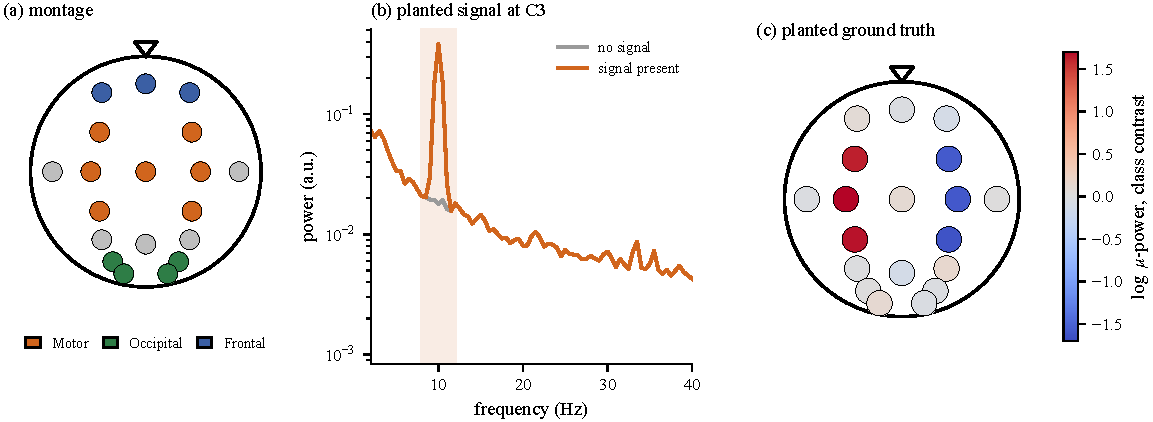
\includegraphics[width=\linewidth]{fig1_simulator.pdf}
\caption{The simulator. (a) The $19$-electrode montage with region labels. (b) Welch
spectra at C3 with and without the planted signal; the $\mu$-band bump is present only
when $s>0$. (c) The planted ground truth: the class contrast in $\mu$ power is confined
to motor channels by construction.}
\label{fig:sim}
\end{figure}

\subsection{Ground truth is operational, not biological}
We are explicit that \cref{eq:signal} is not a cortex. Its value is
\emph{identifiability}: because we placed the signal, we know precisely which
perturbations target something that is there and which target something that is not.
That is exactly the knowledge real data cannot supply, and it is the minimum needed to
measure a false-alarm rate at all. \cref{sec:realbrain} addresses how far the resulting
calibration transfers.

The construction is deliberately easier than biological EEG: background channels are
independent, the carrier is fixed at $10$ Hz, amplitude and onset are constant, and no
volume conduction or artefact process is simulated. Spatial correlation could make a
regional ablation less specific; frequency jitter could spread a true dependence across
bands; and amplitude or onset variation could reduce sensitivity. Absolute rates should
therefore be re-estimated under correlated noise, jitter, and temporal variability
before transfer to another pipeline. The present simulator tests calibration logic, not
biophysical realism.

\section{Controls and Their Operating Characteristics}

\subsection{Definitions}
A control is a map $\mathcal{P}:X\mapsto X'$ that ablates a hypothesised carrier. Band
controls zero a spectral interval,
\begin{equation}
\mathcal{P}_{\text{band}}(X)=\mathcal{F}^{-1}\!\left\{
  \tilde{X}(f)\cdot\ind\!\left[f\notin B\right]\right\},
\label{eq:pband}
\end{equation}
and spatial controls silence an electrode set, $\mathcal{P}_{\mathcal{R}}(X)_{c,t}=0$ for
$c\in\mathcal{R}$. A control \emph{fires} when the induced accuracy drop exceeds a fixed
threshold,
\begin{equation}
\Delta = a\!\left(X_{\text{test}}\right)-a\!\left(\mathcal{P}(X_{\text{test}})\right)
> \tau, \qquad \tau=0.10 .
\label{eq:fire}
\end{equation}
Over repeated datasets we estimate the two rates that define the instrument,
\begin{align}
\text{sensitivity} &= \Pr\!\left(\Delta>\tau \;\middle|\; \text{target present}\right),
\label{eq:sens}\\
\text{false alarm} &= \Pr\!\left(\Delta>\tau \;\middle|\; \text{target absent}\right).
\label{eq:fa}
\end{align}
A control is trustworthy for a given decoder only when \eqref{eq:sens} is high
\emph{and} \eqref{eq:fa} is low \emph{for that decoder}.
The $0.10$ cutoff was fixed before evaluation as a practically conspicuous ten-point
accuracy loss; it is an operating choice, not a physiological constant. We therefore
report its sensitivity below rather than treating it as uniquely correct.

\subsection{A minimal dissociation}
Before the full grid, one controlled comparison isolates the mechanism. We plant the
signal in motor-$\mu$ and build three decoders: \textsc{Focused}, a logistic model on two
features (mean $\mu$ power over left- and right-motor channels); \textsc{Broad}, a
logistic model on $38$ features ($\mu$ and $\beta$ power at all $19$ channels); and
\textsc{Tree}, a random forest on the \emph{identical} $38$ features. Two controls target
the planted signal (remove $\mu$, remove motor) and two target nothing (remove $\beta$,
remove occipital). Results over $15$ datasets appear in \cref{fig:toy}.

\begin{figure}[t]
\centering
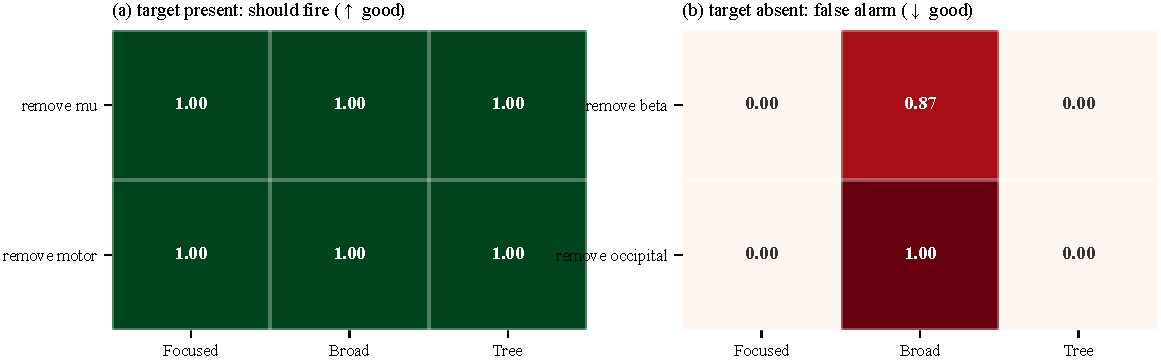
\includegraphics[width=\linewidth]{fig2_toy_fire_rates.pdf}
\caption{Measured fire rates over $15$ simulated datasets. (a) All three decoders detect
the genuinely planted dependence. (b) The linear \textsc{Broad} decoder false-alarms on
$87\%$ of $\beta$ removals and $100\%$ of occipital removals, where no signal exists.
\textsc{Tree} sees the identical $38$ features and never false-alarms.}
\label{fig:toy}
\end{figure}

All three decoders pass the sensitivity test: removing $\mu$ or silencing motor channels
degrades every one of them, as it should. The false-alarm panel dissociates them
completely. \textsc{Broad} fires on $86.7\%$ of $\beta$ removals and $100\%$ of occipital
removals---perturbations that provably destroy no class information---while
\textsc{Focused} and \textsc{Tree} never fire.

The explanation is mechanical and worth stating precisely. A linear model assigns nonzero
weight to essentially every input, so zeroing \emph{any} feature shifts its decision
value and can push trials across the boundary; the drop reflects input perturbation, not
dependence on the ablated carrier. A tree only splits on the features it uses, so
zeroing an unused band or region leaves its decision path untouched. Since \textsc{Broad}
and \textsc{Tree} consume identical inputs, the difference cannot be attributed to what
the decoder can see. Same information, different model class, opposite reliability.

\subsection{Threshold and data-generation sensitivity}
We repeated the minimal experiment on $30$ independently generated train/test datasets
(seeds $1000$--$1029$) and swept $\tau\in\{0.05,0.10,0.15,0.20\}$. \cref{tab:tau}
shows that the qualitative result is threshold-invariant in this range. Each rate pools
the two present-target or two absent-target controls. For \textsc{Broad}, a
dataset-cluster bootstrap gives false-alarm CI $[0.867,0.983]$; for the zero rates, the
dataset-level Wilson upper bound is $0.114$, and unit sensitivity has lower bound
$0.886$. These intervals quantify independent data-generation variability, unlike
retraining the same dataset.

\begin{table}[t]
\centering
\caption{Minimal $19$-channel replication over $30$ independent datasets. FA denotes
false-alarm rate; sensitivity is $1.00$ for all three decoders at every threshold.}
\label{tab:tau}
\begin{tabular}{rrrr}
\toprule
$\tau$ & \textsc{Broad} FA & \textsc{Focused} FA & \textsc{Tree} FA\\
\midrule
0.05 & 0.933 & 0.000 & 0.000\\
0.10 & 0.933 & 0.000 & 0.000\\
0.15 & 0.933 & 0.000 & 0.000\\
0.20 & 0.933 & 0.000 & 0.000\\
\bottomrule
\end{tabular}
\end{table}

\subsection{Measured operating characteristics at scale}
The $19$-channel experiment isolates a mechanism with small named region masks. The full
study expands the same pink-noise and region-specific injection scheme to a standard
$64$-channel montage, mapping motor and occipital masks to their homologous electrodes,
and sweeps $50$ conditions (rhythm $\times$ region $\times$ strength $\times$ confound
$\times$ two signal types). It uses one generated dataset per condition and five model
retrainings on that dataset. Thus retraining variation measures optimisation or resampling
variation, not data-generation uncertainty.

The four families span distinct representations: band-power/logistic regression is a
hand-engineered linear spectral model; CSP/LDA learns supervised spatial filters followed
by a linear rule~\cite{ramoser2000csp}; the forest supplies nonlinear interactions over
engineered features; and EEGNet learns compact temporal and spatial convolutions directly
from trials~\cite{lawhern2018eegnet}. A control is graded only after its decoder clears a
decodability floor. \cref{fig:oc} reports the result.

\begin{figure}[t]
\centering
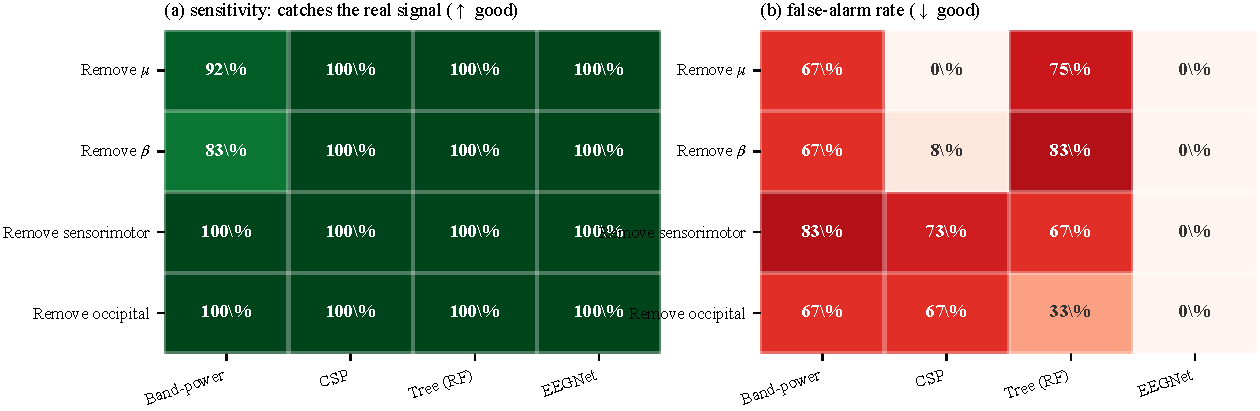
\includegraphics[width=\linewidth]{fig3_operating_characteristics.pdf}
\caption{Measured operating characteristics on the simulator grid. (a) Sensitivity is
high everywhere: all four decoder families detect genuine dependence. (b) False-alarm
rates differ by more than an order of magnitude. Band-power fires on $67$--$83\%$ of
perturbations whose targets are absent; EEGNet essentially never does.}
\label{fig:oc}
\end{figure}

Sensitivity is uninformative---every cell is $83$--$100\%$, so every control detects
real dependence. The discrimination is entirely in the false-alarm panel. Averaged over
probes, the false-alarm rates are $68.8\%$ for band-power, $63.0\%$ for the tree,
$24.7\%$ for CSP, and $1.3\%$ for EEGNet. Because the full grid does not independently
regenerate each condition, these are descriptive rates without data-generation confidence
intervals. They show strong decoder dependence in the tested configuration but should not
be exported as universal constants or a universal factor-of-$50$ contrast.

The tree's position is instructive and refines the toy conclusion. At scale the random
forest does \emph{not} inherit the toy \textsc{Tree}'s immunity: it halves band-power's
occipital false alarms ($33\%$ versus $67\%$) but matches or exceeds it on band controls
($75\%$ on remove $\mu$, $83\%$ on remove $\beta$). Selectivity in the splitting rule
protects against spatial ablation, where irrelevant channels are simply never split on,
but not against band ablation, which corrupts the very features the tree does use. The
failure therefore involves both feature representation and model class. The comparison
is only a partial factorial design: \textsc{Focused} versus \textsc{Broad} varies feature
scope within a linear model, and \textsc{Broad} versus \textsc{Tree} varies model class
at fixed features, but a focused-feature tree is absent. A complete representation
$\times$ model-class factorial is required to estimate their interaction.

\section{Auditing Real Decoders}
We now apply the calibrated battery to decoders trained on PhysioNet
EEGMMIDB~\cite{schalk2004physionet,goldberger2000physiobank} with participant-held-out
evaluation---every subject a decoder is tested on is one it never trained on. All three
real decoders clear the decodability floor (\cref{fig:audit}(b)); the BCI Competition
IV-2a set~\cite{tangermann2012bci} is excluded from the audit because nine participants
render its test underpowered, which is a limitation rather than a result.
The simulator cutoff in Eq.~\eqref{eq:fire} defines event rates; the real audit retains
continuous drops and attaches the corresponding decoder/control reliability rather than
reapplying $\tau$. Population inference must use participants, not trials, as the unit.
Only aggregate held-out accuracies were retained, so participant-level confidence
intervals cannot be reconstructed and the real-data comparison remains descriptive.

\begin{figure}[t]
\centering
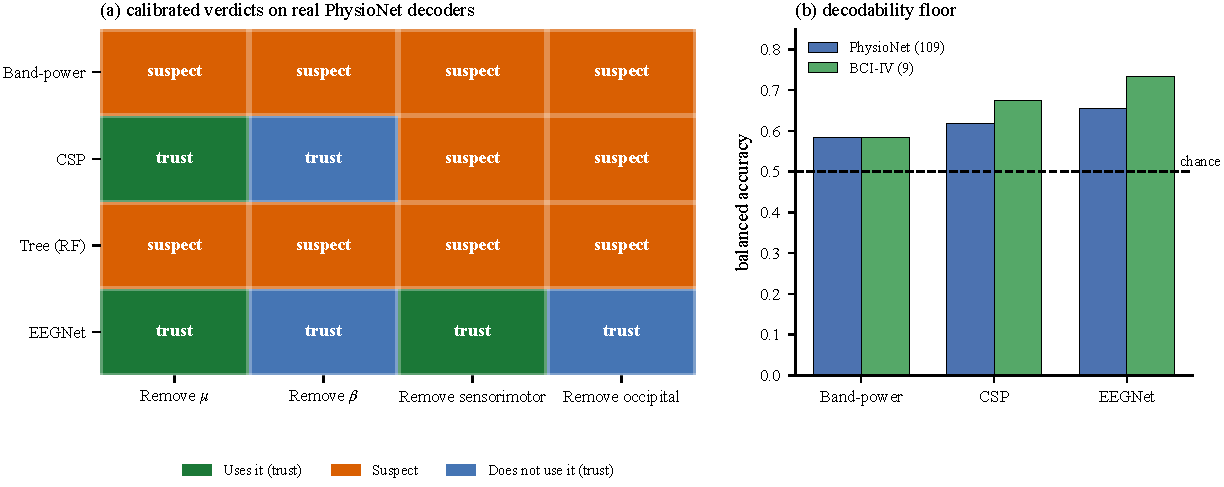
\includegraphics[width=\linewidth]{fig4_calibrated_audit.pdf}
\caption{(a) Calibrated verdicts on real PhysioNet decoders. Each cell attaches the
measured reliability of \cref{fig:oc} to the observed accuracy drop, converting ``the
control fired'' into a trust-weighted statement. Band-power and the tree earn no
trustworthy verdict on any control; EEGNet earns four. (b) Held-out balanced accuracy:
all decoders read motor imagery above chance.}
\label{fig:audit}
\end{figure}

The verdicts are the paper's practical payoff. The four controls produce band-power
drops of $0.03$--$0.08$, and \emph{none} is informative,
because band-power's measured false-alarm rate on each is $67$--$83\%$. The same four
controls applied to EEGNet yield drops of $0.01$--$0.09$ with much lower measured false alarms:
the pattern is consistent with dependence on $\mu$ and sensorimotor channels but not
$\beta$ or occipital channels---four configuration-specific indications, because EEGNet's
false-alarm rate is near zero in the tested grid. CSP is intermediate, trustworthy on the band controls and
suspect on both spatial ones.

An uncalibrated report of the same experiment would have listed eight accuracy drops of
comparable magnitude and drawn eight conclusions. Four of them would have been unfounded.

\section{Validation on Real Brains}
\label{sec:realbrain}
The obvious objection is that all of the above is simulated. Real data cannot in general
settle it, because measuring a false-alarm rate requires knowing that a target is absent,
and on real brains that is unknown---which is why the simulator exists.

There is, however, a way around the impasse: choose a real task whose ground truth
physiology already fixes. Eyes-closed versus eyes-open is the strongest such case in
electroencephalography. Closing the eyes reliably increases occipital alpha, an effect
known since the field's founding~\cite{berkes1929alpha} and characterised in
detail since~\cite{barry2007eoec}. On the resting recordings of the same PhysioNet
participants, we therefore know the discriminative signal is occipital and in the
alpha/$\mu$ band. Controls aimed at that signal \emph{should} fire; controls aimed at
$\beta$, $\theta$, sensorimotor, or frontal targets \emph{should not}.

We decoded eyes-open versus eyes-closed on $34$ subjects (band-power $73\%$, CSP $86\%$
balanced accuracy---a real, strong signal) and graded the controls against that known
truth. \cref{fig:eoec} shows the outcome.

\begin{figure}[t]
\centering
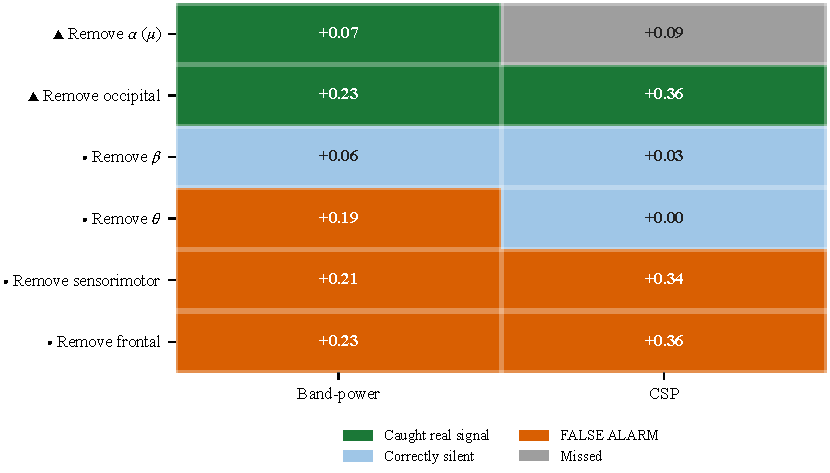
\includegraphics[width=0.72\linewidth]{fig5_real_brain_validation.pdf}
\caption{Real-brain validation on eyes-open versus eyes-closed, $34$ PhysioNet subjects,
where physiology fixes the truth to occipital alpha. Triangles mark controls that should
fire, dots those that should stay silent; cells give the accuracy drop. Band-power
false-alarms on three of four absent targets, CSP on both spatial ones.}
\label{fig:eoec}
\end{figure}

Band-power caught the genuine occipital-alpha dependence---and also fired on $\theta$
removal ($+0.19$), sensorimotor removal ($+0.21$), and frontal removal ($+0.23$),
``detecting'' three dependences that are not there. Its frontal false alarm is
numerically as large as its true occipital detection ($+0.23$ each), so on this decoder
the magnitude of a drop carries no information about whether the target was real. CSP
false-alarmed on both spatial controls, with a frontal drop ($+0.36$) equal to its true
occipital one.

This is a limited simulator-to-real bridge. It corroborates the specificity warning on
a separate task whose physiology is independently known; it does not establish the same
ground truth for motor imagery or validate the numerical simulator rates on real data.
We note the natural confound---volume conduction spreads occipital alpha to
distant electrodes~\cite{nunez2006}---and observe that it strengthens rather than weakens
the conclusion: a control that fires because of field spread is exactly a control that
cannot localise the signal it claims to localise.

\section{Discussion}

\subsection{What the study establishes}
\begin{enumerate}
\item Perturbation controls have measurable, \emph{decoder-conditional} operating
      characteristics: descriptive full-grid false-alarm
      rates range from $1.3\%$ to $68.8\%$ on identical simulated data.
\item Sensitivity is nearly uninformative in this setting; specificity does all the
      discriminating. Studies that report only that a control fired have reported the
      uninformative half.
\item Controlled contrasts implicate both features and model class, but the incomplete
      factorial design does not identify their interaction.
\item Calibration changes how continuous drops are weighted in the descriptive
      PhysioNet audit; participant-level uncertainty remains unmeasured.
\item A known-physiology alpha task corroborates the specificity warning, not the motor-imagery ground truth.
\end{enumerate}

\subsection{What it does not establish}
Simulated ground truth is operational, not biological, so how completely the measured
reliabilities transfer to every recording pipeline remains open---this is the study's
honest crux, not a footnote. The new independent-dataset analysis covers the minimal
$19$-channel comparison only. Each $64$-channel grid condition still rests on one
generated dataset, with five retrainings that measure model variability rather than data
variability; its aggregate rates therefore lack data-generation intervals. Correlated
spatial noise, frequency jitter, amplitude/onset variation, and a complete
representation-by-model factorial remain to be tested. The real-brain confirmation
covers one alpha task, not motor-imagery ground truth. Two older datasets, two-class
motor imagery, and scalp EEG bound the scope. Trials evaluate a decoder, whereas
participants support population claims, and no cortical-causality claim is made.

\subsection{Recommendation}
A perturbation result should not be reported as evidence unless the control's false-alarm
rate has been measured for the decoder in question. Concretely, we recommend that papers
using perturbation controls report, alongside each accuracy drop, the drop induced by at
least one perturbation whose target is known to be absent for that decoder. That single
addition converts an uninterpretable number into an interpretable one, and it is far
cheaper than the calibration grid reported here.

\section{Conclusion}
Perturbation controls are instruments, and instruments require calibration. We measured
the sensitivity and false-alarm rate of band and spatial controls against planted ground
truth and found strong decoder dependence in the tested configurations. The independent
$19$-channel replication is stable across four thresholds, while the larger grid still
needs independent dataset replication. Applying calibration to real-decoder drops changes
their evidential weight, and a known-physiology task corroborates the specificity warning
without establishing motor-imagery causality. The supported conclusion is methodological:
perturbation evidence should be calibrated for its decoder and deployment pipeline.

\section*{Reproducibility}
The accompanying script regenerates the simulator panels and minimal calibration from
\cref{eq:pink,eq:signal} using scikit-learn~\cite{pedregosa2011}. The original minimal
study uses dataset seeds $0$--$14$; each seed generates $60$ training and $60$ test
trials per class, with test seed offset $999$. Logistic models standardise features and
use 	exttt{max\_iter=1000}; the forest uses $200$ trees and seed $0$; $\tau=0.10$.
The threshold analysis uses independent seeds $1000$--$1029$, test offset $100{,}000$,
and $\tau\in\{0.05,0.10,0.15,0.20\}$. CSV files retain aggregate $64$-channel and real
results, but not the per-retraining full-grid seeds or participant-level scores; this
prevents reconstruction of those uncertainty estimates and is a reproducibility limitation.

\bibliographystyle{ACM-Reference-Format}
\bibliography{refs}

\end{document}
